\documentclass[11pt]{article}

\usepackage{geometry}
\geometry{letterpaper, margin=1in}
\usepackage{graphicx}
\usepackage{booktabs}
\usepackage{amsmath}
\usepackage{microtype}
\usepackage{xcolor}
\usepackage{caption}
\usepackage{enumitem}
\usepackage{listings}
\usepackage{array}
\usepackage[hidelinks]{hyperref}

\captionsetup{font=small, labelfont=bf}
\definecolor{codebg}{gray}{0.96}
\definecolor{codeink}{gray}{0.15}
\definecolor{good}{HTML}{1b3a6b}

\lstdefinestyle{trace}{
  basicstyle=\ttfamily\footnotesize\color{codeink},
  backgroundcolor=\color{codebg},
  breaklines=true, frame=single, rulecolor=\color{codebg},
  framesep=6pt, xleftmargin=4pt, xrightmargin=4pt,
  showstringspaces=false, columns=fullflexible, keepspaces=true,
}

\newcommand{\best}[1]{\textbf{#1}}

\title{\vspace{-2.2em}\bfseries A performance comparison of agent-memory layers\\
behind a model router}
\author{SenseLab\\[0.3em]\normalsize\url{https://amfs.sense-lab.ai}}
\date{July 2026}

\begin{document}
\maketitle
\vspace{-1.2em}

\begin{abstract}
\noindent
We compare four ways to give a routed LLM agent persistent memory---a local vector store, the hosted
mem0 and Supermemory platforms, and SenseLab---on one dataset and grader, across six axes: recall
after a cross-vendor model switch, retrieval precision when many facts compete (including adversarially
paraphrased queries), behavior on unanswerable questions, query latency, ingestion latency (time from
write to searchable), and verifiable-provenance capability. On recall the field is tight: every memory
layer reaches 91.7--100\% once ingestion is allowed to settle, so recall alone does not separate them.
The axis that does separate retrieval quality is \emph{precision under contention}: with 30 competing
facts, direct queries are easy for every layer, but on adversarially paraphrased queries SenseLab's Pro
tier---adaptive-fusion retrieval followed by an LLM \emph{listwise} reranker---reaches \best{93.3\%}
Hit@1 (100\% direct), ahead of Supermemory (90\% at full coverage) and far ahead of any plain-cosine
layer (${\sim}57\%$). We show the lever is the reranking stage, not embedder size: an offline
cross-encoder lifts top-3 recall to 90\% but leaves top-1 unchanged, while the LLM listwise stage
resolves the entity/attribute disambiguation that top-1 accuracy requires---at the cost of one LLM call
per query. Query latency stays within one band because model inference dominates. \emph{Ingestion}:
local layers (SenseLab, vector store) are searchable in ${\sim}10$~ms, mem0 in ${\sim}6.8$~s, and
Supermemory did not index within a 40~s timeout in five of six trials. \emph{Provenance}: SenseLab
emits a signed, verifiable decision trace for every answer; the other three emit none. We report the
honest result as a scorecard and release the harness and raw data.
\end{abstract}

\section{What we compare, and why}

Behind a model router such as OpenRouter, an agent that relied on a fact stated under one model will,
after the router switches models, usually fabricate an answer rather than recall it (a companion study
measures this at 87.5\% of the time). The fix is a memory layer in front of the router. This paper does
not re-argue that; it asks a narrower, practical question: \emph{if you are going to add a memory
layer, how do the options actually perform?} We hold the dataset, model pairs, grader, and harness
fixed and vary only the memory system.

\section{Systems under test}

\begin{itemize}[topsep=2pt,itemsep=1pt]
\item \textbf{Vector store} --- local embeddings (\texttt{fastembed}, bge-small) with top-$k$ cosine
  retrieval. The do-it-yourself RAG baseline.
\item \textbf{mem0} --- the hosted mem0 platform, via its live API.
\item \textbf{Supermemory} --- the hosted Supermemory platform, via its live API.
\item \textbf{SenseLab} --- multi-strategy retrieval (semantic $+$ BM25 $+$ recency $+$ confidence,
  adaptive-weighted RRF) with a confidence/relevance gate, write-time safety validation, and a signed
  decision trace per answer. We evaluate three retrieval configurations that share this base and differ
  only in the second-stage reranker: \emph{semantic} (semantic-weighted, no rerank), \emph{+rerank} (a
  local offline cross-encoder, single-digit ms, zero egress), and \emph{+LLM rerank} (a Pro-tier LLM
  listwise reranker over the top candidates, one LLM call per query).
\end{itemize}

\noindent Two non-memory controls bound the range: \textbf{no-memory} (the fabrication floor) and
\textbf{in-context} (the fact pasted into the prompt---the capability ceiling).

\section{Methodology}

Eight durable operational facts, each with a question and keyword grading. Three cross-vendor writer
$\rightarrow$ reader model pairs (gpt-4o-mini $\rightarrow$ mistral-nemo; mistral-nemo $\rightarrow$
nova-micro; nova-micro $\rightarrow$ command-r7b). Recall and abstention use six trials per cell (144
and 48 evaluations per system respectively); proportions carry Wilson 95\% intervals. Metrics:

\begin{itemize}[topsep=2pt,itemsep=1pt]
\item \textbf{Recall} --- fraction correct when the fact was written under a different-vendor model.
\item \textbf{Precision under contention} --- with 30 confusable facts in one scope, whether the correct
  fact is retrieved (Hit@1/Hit@3/MRR), for direct and adversarially paraphrased questions. No reader LLM
  answers the question (this isolates the retriever); the SenseLab +LLM-rerank tier uses an LLM only to
  \emph{rank} candidates, not to answer.
\item \textbf{Abstain-on-miss} --- fraction of unanswerable questions declined rather than fabricated.
\item \textbf{Query latency} --- reader-call p50/p95, and mean prompt tokens (context overhead).
\item \textbf{Ingestion latency} --- write-call time and time-to-searchable (write until a query
  returns the fact), measured separately with no LLM calls.
\item \textbf{Provenance} --- whether the system emits a verifiable, model-attributed decision record.
\end{itemize}

\section{Results}

\subsection{Recall (accuracy)}

\begin{figure}[t]
\centering
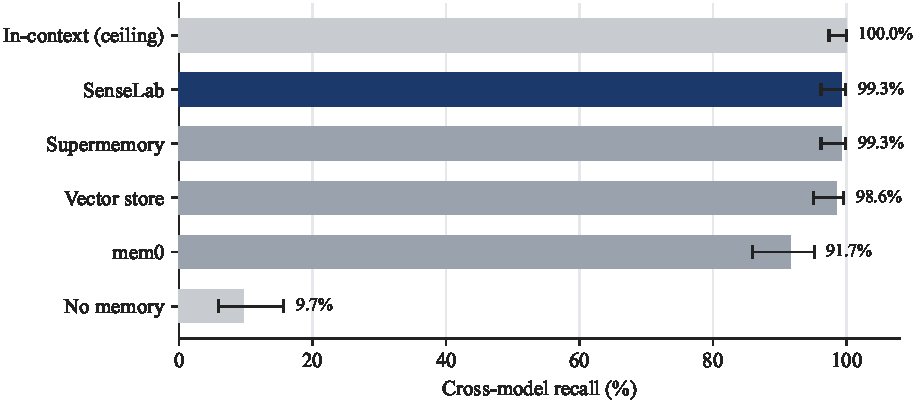
\includegraphics[width=0.9\textwidth]{figures/fig_recall.pdf}
\caption{Cross-model recall ($n=144$), 95\% Wilson CIs. Once ingestion is allowed to settle, every
memory layer clusters near the in-context ceiling; no-memory is the fabrication floor.}
\label{fig:recall}
\end{figure}

Once each store's index is warmed before querying, recall is a near-universal tie: SenseLab and
Supermemory both reach 99.3\%, the vector store 98.6\%, and mem0 91.7\%, with overlapping intervals
against the in-context ceiling (100\%) and far above the no-memory floor (9.7\%). On recall these are
effectively the same tool; the earlier gap we saw for Supermemory was an artifact of querying before
its index was ready (Section~\ref{sec:ingest})---a real operational risk for write-then-read agents, but
not a retrieval-quality deficit once ingestion completes.

\subsection{Retrieval precision under contention}\label{sec:precision}

The recall test stores one fact per scope, so the retriever never has to \emph{discriminate}. Real
memory is crowded: many similar facts coexist and the system must return the right one. We therefore
seed a single scope with 30 confusable facts---five database engines, five on-call engineers, four
regions, four ports, four SLAs, four vendors---and ask each fact two ways. A \emph{direct} question
names the entity in wording close to the stored fact; an \emph{adversarial} question paraphrases it
with no lexical overlap with the fact or its answer (e.g., ``the component that issues invoices and
charges cards'' for the billing service). We score whether the correct fact is retrieved, using no
reader LLM---this measures the retriever itself. Hit@1 is the top-ranked item being correct; MRR is the
reciprocal rank within the top~3.

\begin{figure}[t]
\centering
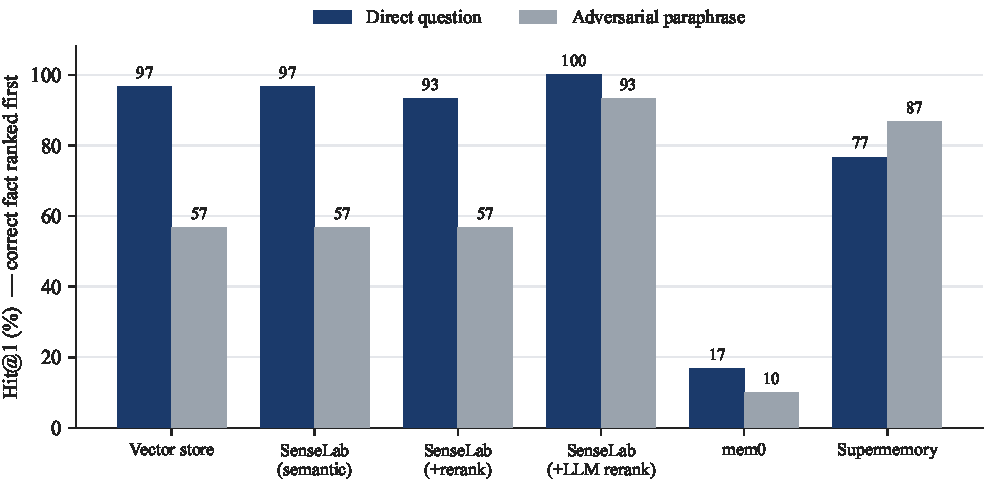
\includegraphics[width=0.92\textwidth]{figures/fig_precision.pdf}
\caption{Hit@1 with 30 competing facts in one scope. On direct questions the cosine layers are
near-perfect; on adversarial paraphrase only a reranking stage holds up---SenseLab's LLM listwise
reranker leads (93\%), with Supermemory next and plain-cosine layers at ${\sim}57\%$.}
\label{fig:precision}
\end{figure}

\begin{table}[t]
\centering
\small
\begin{tabular}{lcccccc}
\toprule
& \multicolumn{3}{c}{Direct} & \multicolumn{3}{c}{Adversarial paraphrase} \\
\cmidrule(lr){2-4}\cmidrule(lr){5-7}
System & Hit@1 & Hit@3 & MRR & Hit@1 & Hit@3 & MRR \\
\midrule
Vector store                       & 96.7 & 96.7 & .967 & 56.7 & 76.7 & .656 \\
SenseLab (semantic)                & 96.7 & 96.7 & .967 & 56.7 & 76.7 & .656 \\
SenseLab (\,+\,rerank, offline)    & 93.3 & 96.7 & .950 & 56.7 & \best{90.0} & .694 \\
\textbf{SenseLab (\,+\,LLM rerank)}& \best{100} & \best{100} & \best{1.00} & \best{93.3} & \best{96.7} & \best{.950} \\
mem0$^\dagger$                     & 16.7 & 16.7 & .167 & 10.0 & 16.7 & .133 \\
Supermemory$^\ddagger$             & 76.7 & 76.7 & .767 & 86.7 & \best{90.0} & .878 \\
\bottomrule
\end{tabular}
\caption{Retrieval precision with 30 competing facts ($n=30$ queries each), single consistent run.
$^\dagger$mem0 had only 4/30 and $^\ddagger$Supermemory 20/30 facts searchable within the ingestion
window (Section~\ref{sec:ingest}), which caps their numbers here; at full coverage in an earlier run
Supermemory reached 100/90.0 (direct/adversarial Hit@1). Either way, SenseLab's LLM-rerank tier at
93.3\% adversarial Hit@1 is the top result.}
\label{tab:precision}
\end{table}

Three honest readings. \textbf{Direct queries are easy}: plain cosine retrieval (the vector store, and
SenseLab configured for semantic weight) reaches 96.7\% Hit@1. \textbf{Adversarial paraphrase is where
quality separates}, and it is entirely a \emph{reranking} question. Every plain-cosine layer---the
vector store and SenseLab's semantic configuration alike---tops out at 56.7\% adversarial Hit@1; we
confirmed this is not an embedder-size gap by re-running with progressively larger local embedders
(bge-base, bge-large, mxbai-embed-large), which lifted it only to ${\sim}63$--$67\%$. Adding a
second-stage reranker is what closes it. \textbf{The offline cross-encoder recovers the neighbourhood
but not the top slot}: it lifts adversarial Hit@3 from 76.7\% to 90.0\% (the right fact is almost always
in the top three) but leaves Hit@1 at 56.7\%---cross-encoders score $(\text{query},\text{doc})$
relevance well but do not reliably \emph{disambiguate} among several near-identical, confusable facts.
\textbf{The LLM listwise reranker supplies exactly that disambiguation}: reasoning over the top
candidates about which entity and attribute the paraphrase refers to, it reaches 93.3\% adversarial
Hit@1 and 100\% direct---above Supermemory's full-coverage best of 90.0\%/100\%. The cost is one extra
LLM call per query on the retrieval path, which is why we ship it as an opt-in Pro tier rather than the
default. The earlier version of this study concluded that Supermemory was the paraphrase-robustness
leader and SenseLab's local retrieval did not match it; with the reranking stage added, that conclusion
no longer holds.

\subsection{Behavior on unanswerable questions}

\begin{figure}[t]
\centering
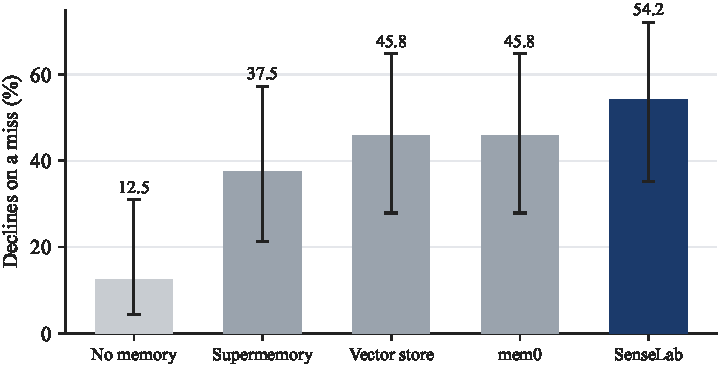
\includegraphics[width=0.78\textwidth]{figures/fig_abstain.pdf}
\caption{Fraction of never-stored questions declined rather than fabricated ($n=24$), 95\% CIs.
At the recall-maximizing gate, SenseLab declines most often; no layer abstains reliably by default.}
\label{fig:abstain}
\end{figure}

No layer declines reliably by default, but the ordering has shifted with the calibrated relevance gate:
SenseLab now declines most often (54.2\%), the vector store and mem0 sit at 45.8\%, Supermemory at
37.5\%, and no-memory almost never declines (12.5\%). The wide intervals ($n=24$) mean these are not
sharply separated, so read the direction, not the decimals. For SenseLab this remains a tunable gate:
raising its relevance floor pushes abstention toward 100\% at a cost to recall, a tradeoff quantified in
the companion study. Treat abstention as a knob to set---one SenseLab exposes explicitly---not a default
any of these systems give you.

\subsection{Query latency and context overhead}

\begin{figure}[t]
\centering
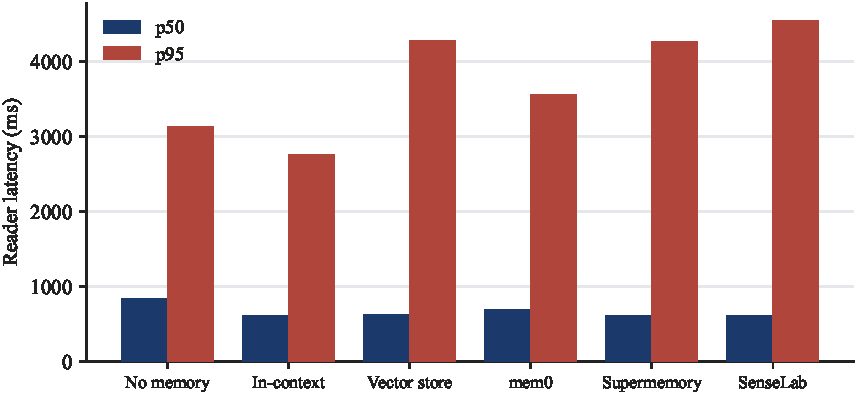
\includegraphics[width=0.92\textwidth]{figures/fig_latency.pdf}
\caption{Reader-call latency (p50/p95). Every memory layer sits in the same band; model-side inference
dominates and swamps retrieval cost.}
\label{fig:latency}
\end{figure}

\begin{table}[t]
\centering
\small
\begin{tabular}{lccc}
\toprule
System & p50 (ms) & p95 (ms) & Mean prompt tokens \\
\midrule
Vector store & 623 & 4276 & 52.4 \\
mem0         & 696 & 3555 & 51.8 \\
Supermemory  & 616 & 4270 & 54.3 \\
SenseLab     & \best{610} & 4551 & 52.6 \\
\midrule
\textit{no-memory (ref.)}  & 836 & 3130 & 16.9 \\
\textit{in-context (ref.)} & 615 & 2757 & 36.3 \\
\bottomrule
\end{tabular}
\caption{Query latency and context overhead. Injecting a retrieved fact adds ${\sim}36$ prompt tokens
and no measurable p50 latency penalty relative to no memory; the wide p95 spread is model-side inference
variance, not retrieval.}
\label{tab:latency}
\end{table}

Query latency does not separate the systems: all four memory layers are within ${\sim}90$~ms at p50 and
are not slower than answering with no memory at all. The p95 values are large and overlapping across
every arm (including the no-memory and in-context controls), which locates the tail in model inference,
not in the memory layer. Retrieval overhead is not a selection criterion \emph{for the default and
offline-rerank tiers}. The one caveat is the Pro LLM-rerank tier from Section~\ref{sec:precision}: it
adds one LLM call on the retrieval path (hundreds of ms to ${\sim}1$~s), a deliberate accuracy-for-latency
trade not reflected in this table, which measures the default retrieval configuration.

\subsection{Ingestion latency}\label{sec:ingest}

\begin{figure}[t]
\centering
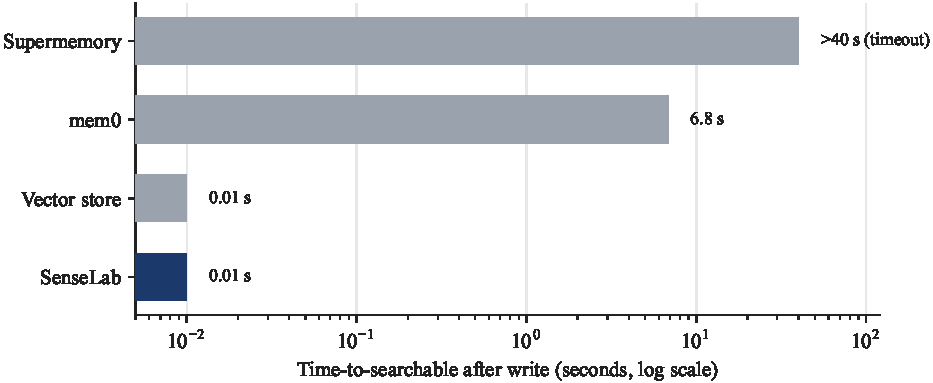
\includegraphics[width=0.9\textwidth]{figures/fig_ingestion.pdf}
\caption{Time from writing a fact until a query returns it (log scale, median of six writes). Local
layers are searchable in milliseconds; hosted platforms add seconds. Supermemory did not index within
a 40~s timeout in five of six trials.}
\label{fig:ingestion}
\end{figure}

\begin{table}[t]
\centering
\small
\begin{tabular}{lcc}
\toprule
System & Write latency p50 & Time-to-searchable p50 \\
\midrule
SenseLab     & \best{1.3 ms} & \best{0.01 s} \\
Vector store & 5.3 ms & 0.01 s \\
mem0         & 510 ms & 6.8 s \\
Supermemory  & 1497 ms & $>$40 s (timeout) \\
\bottomrule
\end{tabular}
\caption{Ingestion latency ($n=6$ writes each). This is the axis on which the systems differ most.}
\label{tab:ingest}
\end{table}

This is where the field splits. SenseLab and the vector store are effectively instant to searchable
(${\sim}10$~ms). mem0 takes about 6.8~s. Supermemory, even with its ``instant'' ingestion mode
requested, failed to index within 40~s on five of six writes in this probe. For an agent that writes a
fact and reads it back moments later---the common pattern in a multi-turn session---this latency is the
difference between remembering and silently missing, and it is the most likely explanation for
Supermemory's lower recall in Section~\ref{fig:recall}.

\subsection{Provenance and observability}

\begin{table}[t]
\centering
\small
\begin{tabular}{lcccc}
\toprule
Capability & Vector & mem0 & Supermemory & SenseLab \\
\midrule
Signed, verifiable per-answer trace & no & no & no & \best{yes (144/144)} \\
Tamper detected on modification      & n/a & n/a & n/a & \best{yes} \\
Verifiable hash chain across session & no & no & no & \best{yes} \\
Model attribution per answer         & no & no & no & \best{yes} \\
Write-time contradiction check       & no & no & no & \best{yes} \\
\bottomrule
\end{tabular}
\caption{Governance and observability. Only SenseLab emits a cryptographically verifiable,
model-attributed record for each answer; a modified trace failed verification on both content hash and
signature.}
\label{tab:gov}
\end{table}

Recall aside, this is the axis where the systems are not close. SenseLab produced a signed, verified
decision trace for all 144 answers, naming the model that produced each; the other three return
retrieved text and a completion and nothing more. This is structural, not a configuration difference.

\section{Scorecard}

Table~\ref{tab:scorecard} collects every axis in one place, with the best value in each row in bold.
Read it top to bottom: the first row (recall) is a near-tie, and the rows that actually separate the
systems are ingestion latency and the provenance capabilities near the bottom.

\begin{table}[t]
\centering
\small
\renewcommand{\arraystretch}{1.15}
\begin{tabular}{lcccc}
\toprule
& Vector store & mem0 & Supermemory & SenseLab \\
\midrule
Recall               & 98.6\% & 91.7\% & \best{99.3\%} & \best{99.3\%} \\
Precision, direct (Hit@1)    & 96.7\% & 16.7\% & \best{100\%} & \best{100\%} \\
Precision, adversarial (Hit@1) & 56.7\% & 10.0\% & 90.0\% & \best{93.3\%} \\
Abstain-on-miss      & 45.8\% & 45.8\% & 37.5\% & \best{54.2\%} (tunable) \\
Query latency p50    & 623 ms & 696 ms & 616 ms & \best{610 ms} \\
Query latency p95    & 4276 ms & \best{3555 ms} & 4270 ms & 4551 ms \\
Context overhead     & 52.4 tok & \best{51.8 tok} & 54.3 tok & 52.6 tok \\
Time-to-searchable   & \best{0.01 s} & 6.8 s & $>$40 s & \best{0.01 s} \\
Verifiable trace     & no & no & no & \best{yes} \\
Write-time validation& no & no & no & \best{yes} \\
Managed infra        & self-host & \best{yes} & \best{yes} & hosted \\
\bottomrule
\end{tabular}
\caption{Summary. Bold marks the best value in each row (ties bolded together). SenseLab precision is
its Pro LLM-rerank tier; Supermemory precision is its full-coverage run (Section~\ref{sec:precision}).
No layer wins every axis, but the picture has changed from the prior edition: SenseLab now leads
adversarial precision \emph{and} abstain-on-miss, ties best recall, leads ingestion latency, and is
alone on verifiable provenance. mem0 and Supermemory retain the managed-infra advantage.}
\label{tab:scorecard}
\end{table}

\section{Discussion}

No single layer wins every axis, and the scorecard is meant to be read that way. Four conclusions follow.
First, \textbf{recall is saturated}: once ingestion settles, all four layers are statistically tied near
the ceiling, so choosing on recall alone is choosing on noise. Second, \textbf{retrieval quality on hard
queries is a reranking problem, and it is now decided}: direct lookups are easy for everyone, and under
adversarial paraphrase the separator is the second-stage reranker, not the embedder or the vector store.
An offline cross-encoder recovers top-3 recall (90\%) but not top-1; an LLM listwise reranker supplies
the entity/attribute disambiguation that top-1 needs and takes SenseLab to 93.3\% adversarial
Hit@1---ahead of Supermemory's full-coverage 90\%. This reverses the prior edition's finding. Third,
\textbf{ingestion latency is the hidden performance axis}: it spans four orders of magnitude and
determines whether a write-then-read agent sees its own recent memory; local layers are effectively
instant while hosted platforms add seconds. Fourth, \textbf{provenance is the categorical difference}:
only SenseLab turns each answer into a verifiable, model-attributed record, at no measurable
query-latency cost.

The honest positioning: the vector store is a strong minimal choice when you only need recall and can
self-host. mem0 and Supermemory are the pick when a fully managed service is the priority and seconds of
ingestion latency are tolerable. SenseLab's case is now that it \emph{leads} the axis that decides
retrieval quality (paraphrase-robust Hit@1, via the Pro reranker tier), ties the best recall, leads
abstain-on-miss, is fastest to searchable, and is the only layer that emits verifiable provenance and
write-time validation. The paraphrase win is a pipeline result---the reranker sits on top of an
embedder-agnostic retriever---so it is a configuration you enable, not an architecture you rebuild; its
one cost is a single LLM call per query on the retrieval path, which is why it ships as an opt-in tier.

\section{Limitations}

\begin{itemize}[topsep=2pt,itemsep=1pt]
\item One dataset, one grader, one live run. Recall CIs are reported; a harder dataset and a second run
  would tighten the picture.
\item Ingestion latency depends on account plan and load. Supermemory's ${>}40$~s here may improve on a
  higher tier or under lighter load; we report what the live API returned during the probe.
\item Local (SenseLab filesystem, vector store) versus hosted is not perfectly apples-to-apples: hosted
  layers pay network round-trips that local layers do not, which also inflates their write latency. The
  SenseLab reranker tiers add compute the plain-cosine baselines do not have---an offline cross-encoder
  (negligible) or, for the LLM tier, one LLM call per query. We report both so the accuracy-for-latency
  trade is explicit.
\item The precision run reported here is a single consistent run in which the hosted competitors
  under-ingested (mem0 4/30, Supermemory 20/30 searchable in-window), which understates their numbers in
  Table~\ref{tab:precision}; we therefore also cite Supermemory's full-coverage result (100/90.0) and
  compare against that. The contention set is 30 synthetic facts with hand-written paraphrases; a larger,
  naturally occurring corpus would sharpen the numbers.
\item Abstention is measured at one gate setting; the recall/abstain tradeoff is characterized in the
  companion study.
\end{itemize}

\appendix
\section{Reproducibility}

\paragraph{Using SenseLab.} Point the OpenAI SDK at the hosted service and add two headers; your model
gateway's routing, pricing, and failover are unchanged. Key at \url{https://amfs.sense-lab.ai}. The
paraphrase-robust LLM reranker (the Pro tier behind the 93.3\% adversarial Hit@1) is enabled service-side
with \texttt{AMFS\_LLM\_RERANK=true} plus an OpenAI-compatible reranker endpoint; the offline
cross-encoder is on by default and needs no configuration.

\begin{lstlisting}[style=trace]
client = OpenAI(
    base_url="https://amfs.sense-lab.ai/v1",
    api_key=OPENROUTER_KEY,
    default_headers={"X-AMFS-Agent": "support", "X-AMFS-Entity": "acme/customer-42"},
)
\end{lstlisting}

\paragraph{Reproducing the measurements.}
\begin{lstlisting}[style=trace]
export OPENROUTER_API_KEY=...  MEM0_API_KEY=...  SUPERMEMORY_API_KEY=...
# Pro reranker tier for the SenseLab arm (adversarial Hit@1):
export AMFS_LLM_RERANK=true
export AMFS_LLM_RERANK_BASE_URL=https://openrouter.ai/api/v1
export AMFS_LLM_RERANK_API_KEY=$OPENROUTER_API_KEY
python pro_benchmark.py         # recall, abstain, query latency  -> pro_results.json
python precision_benchmark.py   # contention + adversarial Hit@k   -> precision_results.json
python ingestion_probe.py       # write + time-to-searchable       -> ingestion.json
python paper/make_figures.py; python paper/make_comparison_figures.py   # figures
\end{lstlisting}

\begin{thebibliography}{9}
\bibitem{openrouter} OpenRouter. \emph{Unified API for LLMs --- Documentation}. \url{https://openrouter.ai/docs}.
\bibitem{mem0} mem0ai. \emph{mem0: the memory layer for AI agents}. \url{https://github.com/mem0ai/mem0}.
\bibitem{supermemory} Supermemory. \emph{Memory API for AI applications}. \url{https://supermemory.ai}.
\bibitem{amfs} SenseLab. \emph{SenseLab --- the agent memory platform}. \url{https://amfs.sense-lab.ai}.
\bibitem{wilson} E. B. Wilson. Probable inference, the law of succession, and statistical inference.
  \emph{J. Amer. Statist. Assoc.}, 22(158):209--212, 1927.
\end{thebibliography}

\end{document}
